\section{Grundlagen}
\subsection{Problemstellung}
Durch zahlreiche vorangegangene Studienarbeiten wurden bereits viele grundlegende
Funktionen des Hochregallagers implementiert.
Hierzu gehören unter anderem:

\begin{itemize}
    \item automatisiertes Einlagern,
    \item manuelles Auslagern,
    \item sowie die \textbf{RFID-Materialerkennung}.
\end{itemize}

Diese Funktionen bleiben im Rahmen dieser Arbeit bestehen und sind nicht Hauptbe
standteil der weiteren Bearbeitung.
Der Fokus der vorliegenden Studienarbeit liegt vielmehr auf der Integration zusätzlicher
\textbf{Sicherheitskomponenten}, der Fertigstellung der \textbf{RFID-Materialerkennung} sowie der
\textbf{Überarbeitung bzw. Umstellung des SPS-Programms} auf die Programmiersprache
\textbf{Structured Text (ST)}.
Für den sicheren Betrieb eines Hochregallagers sind verschiedene Schutzmecha
nismen erforderlich, um Gefahren beim Eingriff in den laufenden Prozess zu vermeiden.
Einige dieser Maßnahmen wurden bereits in früheren Arbeiten umgesetzt.
Ein wesentliches, bislang fehlendes Sicherheitselement ist jedoch eine Lichtschranke,
die sich unmittelbar vor dem Lagerbereich befindet. Diese soll im Rahmen dieser Arbeit
in das Steuerungsprogramm integriert werden, um potenzielle Gefährdungen bei manu
ellen Eingriffen während des Betriebs zu verhindern.


Darüber hinaus ist zur Gewährleistung eines fehlerfreien Ablaufs während der Ma
terialerkennung die Funktionalität der RFID-Prüfung zu analysieren, zu optimieren und
gegebenenfalls zu vervollständigen.
Ein weiterer wichtiger Aspekt betrifft die verwendete Programmiersprache des SPS
Systems. In den bisherigen Studienarbeiten wurde überwiegend die grafische Program
miersprache \textbf{FBS (Funktionsbausteinsprache)} eingesetzt. Diese bietet den Vorteil
einer einfachen, blockorientierten Programmstruktur, stößt jedoch bei komplexeren
Anwendungen schnell an ihre Grenzen.
Aus Gründen der Übersichtlichkeit, Wartbarkeit und Fehlersuche soll das bestehende
Programm daher in die textbasierte Programmiersprache \textbf{ST (Structured Text)} übertra
gen werden.
Abschließend lässt sich festhalten, dass die wesentlichen Funktionen des bestehenden
Hochregallagers bereits implementiert sind. Trotzdem bestehen noch Optimierungs
potenziale im Hinblick auf Sicherheit, Struktur und Programmiermethodik. Um die
geplanten Maßnahmen gezielt umsetzen zu können, ist es erforderlich, den aktuellen
technischen Aufbau und die bestehende Programmstruktur zunächst detailliert zu ana
lysieren. Im folgenden Abschnitt „Stand der Technik“ werden daher die vorhandenen
Komponenten und deren Funktion genauer betrachtet, um eine fundierte Grundlage für
die anschließende Überarbeitung zu schaffen

\subsection{Stand der Technik}
\subsubsection{Aufbau des Hochregallagers}
Bei der zu optimierenden Anlage handelt es sich um ein \textbf{Modell-Hochregallager} im
Laborraum H001 der \textbf{Dualen Hochschule Baden-Württemberg} am Campus Fried
richshafen. Diese dient dazu, den Studierenden bei vertretbaren Anschaffungskosten
ein Modell einer \textbf{modernen Hochregalanlage}, wie sie auch in zahlreichen \textbf{Industriebetrieben} zu finden ist, zu bieten.
Um den Aufbau der Anlage fachgerecht erklären zu können, ist die Definition eines
\textbf{Koordinatensystems} für die Bewegung der \textbf{Einlagerungsvorrichtung} notwendig:


\begin{figure}[H]
        \centering
        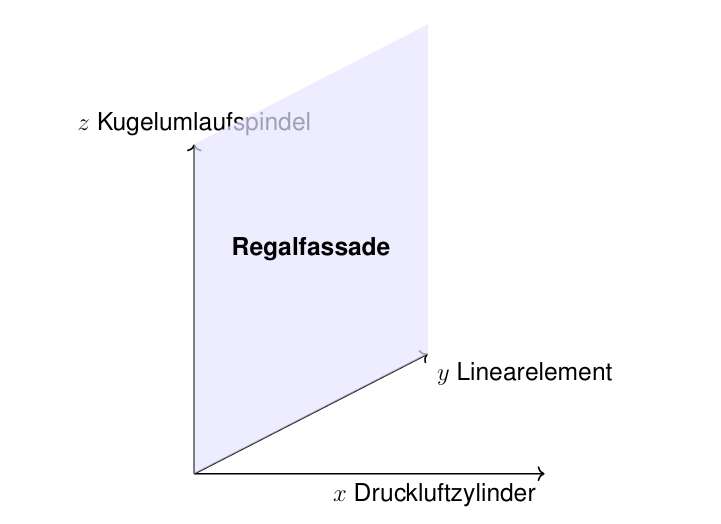
\includegraphics[width=400px]{images/KoordinatensystemAufbau.png}
        \caption{Schaubild zum Systemaufbau des Hochregallagers}
        \label{fig:koordsysaufbau}
    \end{figure}

\begin{itemize}
    \item x-Achse-> Bewegung des Trägers in das Hochregal
    \item y-Achse-> Bewegung des Trägers in Horizontale entlang der Regalstruktur
    \item z-Achse-> Bewegung des Trägers in Vertikale entlang der Regalstruktur
\end{itemize}




Die \textbf{Förder- und Bewegungssysteme} der Modell-Hochregalanlage stellen das zentrale
Element zur Realisierung \textbf{automatisierter Lagerprozesse} dar. Die Anlage ist so kon
zipiert, dass sie die \textbf{Ein- und Auslagerung} von Lagergütern in einem mehrstöckigen
Regalsystem ermöglicht. Die Bewegungsachsen werden in drei Dimensionen unterteilt:
\textbf{horizontal, vertikal} und die eigentliche \textbf{Einlagerbewegung}.


Die \textbf{horizontale Verfahrbewegung} (y-Achse) des Regalbediengeräts erfolgt über ein
\textbf{Linearelement}, das entlang einer \textbf{Führungsschiene} verläuft. Das Linearsystem basiert
auf einem \textbf{motorgetriebenen Schlitten}, welcher präzise Positionierungen entlang der
Regalfassade ermöglicht. Die Führungsschiene gewährleistet eine stabile und reibungs
arme Bewegung, während der Antrieb über einen \textbf{Schrittmotor} erfolgt, der über eine
\textbf{Steuerungseinheit} angesteuert wird. Die Positionserfassung wird gegenwärtig durch
\textbf{Timer im Steuerungsprogramm} realisiert. Die Positionierung der \textbf{Endschalter} erfolgt
ausschließlich am Ende der Achsen.


Die \textbf{vertikale Bewegung} (z-Achse) wird durch eine \textbf{Kugelumlaufspindel} realisiert,
die eine hohe Positioniergenauigkeit und mechanische Effizienz bietet. Die Spindel ist
mit einem \textbf{rotatorischen Antrieb} gekoppelt, der die Drehbewegung in eine lineare
\textbf{Hubbewegung} umsetzt. Die Verwendung von \textbf{Kugelumlaufmuttern} führt zu einer
Minimierung der Reibung und einer Erhöhung der Tragfähigkeit, was insbesondere bei
mehrstöckigen Regalsystemen vorteilhaft ist. 
Die vertikale Führung erfolgt über ein sta
biles Profil, das die Bewegung des Hubsystems stabilisiert und ein Verkanten verhindert.



Die eigentliche \textbf{Einlagerung des Lagerguts} (x-Achse) erfolgt mittels eines \textbf{Druck
luftzylinders}. Der Zylinder ist am Regalbediengerät montiert und fährt bei Erreichen
der Zielposition aus, um das Lagergut in das vorgesehene Fach zu überführen. Die
Wahl eines pneumatischen Systems ermöglicht eine schnelle und kraftvolle Bewegung,
die unabhängig von der elektrischen Steuerung arbeitet und sich gut für wiederholte,
gleichförmige Bewegungsabläufe eignet. Die Steuerung des Zylinders erfolgt durch ein
\textbf{Magnetventil}, das durch die SPS angesteuert wird.
Die \textbf{Sensorik und Steuerungseinheiten} der Modell-Hochregalanlage übernehmen
zentrale Aufgaben zur Gewährleistung eines sicheren und präzisen Betriebs. Sie er
möglichen sowohl die \textbf{Positionsbestimmung} der beweglichen Komponenten als auch
die \textbf{Identifikation der Lagergüter} und die \textbf{Prozesssteuerung}.
Zur Erfassung der Endstellungen der horizontalen und vertikalen Bewegungsachsen
werden mechanische \textbf{Endschalter} verwendet. Diese sind jeweils an den Begrenzungs
punkten der Lineareinheit sowie der Kugelumlaufspindel angebracht und dienen der
sicheren Detektion der maximalen Verfahrwege. Das Erreichen einer Endlage löst
den entsprechenden Schalter aus und führt zur Übertragung eines Signals an die
Steuerungseinheit. Diese Vorgehensweise verhindert ein Überfahren der mechanischen
Grenzen und gewährleistet den Schutz der Anlage vor potenziellen Schäden.



Die \textbf{Materialerfassung} erfolgt mittels eines \textbf{RFID-Systems}, welches sich aus einer
\textbf{RFID-Antenne} und entsprechenden \textbf{Transpondern} zusammensetzt. Jedes Element
des Lagers ist mit einem \textbf{RFID-Tag} ausgestattet, der eine eindeutige Identifikation
ermöglicht. Die Positionierung der Antenne erlaubt es, beim Ein- oder Auslagern eines
Artikels dessen Transponder auszulesen. Die erfassten Daten werden unmittelbar an die
Steuerung übermittelt und dort verarbeitet. Das berührungslose Identifikationsverfahren
ermöglicht eine schnelle und fehlerfreie Zuordnung der Lagergüter.



Die zentrale Steuerung der Anlage erfolgt mittels einer \textbf{SPS vom Typ Siemens S7-1511},
welche sämtliche Bewegungsabläufe, Sensorrückmeldungen und Aktorsteuerungen
koordiniert. Die SPS ist über ein \textbf{HMI (Human-Machine Interface)} mit dem Bedienper
sonal verbunden, wodurch eine intuitive Bedienung und Visualisierung der Anlagenzu
stände ermöglicht wird. Über das HMI können Betriebsmodi gewählt, Lagerprozesse
gestartet und Diagnosedaten eingesehen werden.




\subsubsection{Speicherprogrammierbare Steuerungen}
Die \textbf{Speicherprogrammierbare Steuerung} (SPS) stellt ein zentrales Element moderner
industrieller Automatisierung dar.Sie ermöglicht die flexible, softwarebasierte Steuerung
technischer Prozesse und ersetzt zunehmend klassische \textbf{verbindungsprogrammierte
Steuerungen} wie Relais-und Schütztechnik. Insbesondere die SPS-Systeme der
Siemens AG, unter dem Markennamen SIMATIC bekannt, nehmen eine führende Rolle
in der industriellen Praxis ein.
Im folgenden eine Gegenüberstellung von VPS und SPS:

\begin{center}
    % Erzeugt eine normale Tabellenbeschriftung ohne \begin{table}

    \begin{tabular}{|p{4cm}|p{6cm}|p{6cm}|}
        \hline
            \textbf{Kriterium}  & \textbf{SPS (Speicherprogrammierbare Steuerung)} & \textbf{VPS (Verbindungsprogrammierte Steuerung)} \\
            \hline
            \textbf{Flexibilität}& Hohe Flexibilität durch einfache Softwareänderung& Geringe Flexibilität,Änderungen erfordern Hardwareeingriffe\\
            \hline
            \textbf{Programmierung} &  Softwarebasiert über Programmiersprachen(z.B.KOP, FUP,SCL)& Hardwarebasiert durch Verdrahtung von Relais und Schützen\\
            \hline
            \textbf{Fehlersuche}& Komfortable Diagnosefunktionen über Softwaretools& Fehlersuche oft manuell und zeitaufwendig\\
            \hline
            \textbf{Platzbedarf}& Kompakte Bauweise, platzsparend & Großer Platzbedarf durch viele Einzelkomponenten\\
            \hline
            \textbf{Kosten bei Änderungen}& Geringe Kosten, da keine Hardwareänderungnötig& Hohe Kosten durch Umbau und neue Komponenten\\
            \hline
            \textbf{Wartung}&Zentralisiert und soft waregestützt& Dezentral und hardwareintensiv  \\
            \hline
            \textbf{Komplexität der Steuerung}& Geeignet für komplexe und vernetzte Systeme & Nur für einfache Steuerungsaufgaben geeignet   \\
            \hline
            \textbf{Zukunftsfähigkeit}& Industrie 4.0-fähig, IoT-Integration möglich & Veraltet,kaum kompatibel mit modernen Systemen \\
            \hline
    \end{tabular}

    \captionof{table}{Vergleich zwischen SPS und VPS hinsichtlich technischer und wirtschaftlicher Kriterien; Quelle:[21]}
    \label{tab:VergleichSpsVps}
\end{center}


Die SIMATIC-Reihe von Siemens ist in zwei Produktlinien gegliedert,welche sich
hauptsächlich in ihren Anwendungsbereichen unterscheiden. Die S7-1200 ist für die
Realisierung kompakter Automatisierungslösungen konzipiert,wohingegen die S7-1500
erweiterte Funktionen für die Bewältigung komplexer Steuerungsaufgaben in vernetzten
Produktionsumgebungen bietet. Die Funktionsweise beider Systeme ist durch das
EVA-Prinzip (Eingabe– Verarbeitung– Ausgabe) determiniert. Die Bereitstellung der
Eingangssignale erfolgt durch Sensoren, deren Signale durch die CPU verarbeitet und
anschließend durch Aktoren umgesetzt werden


\begin{figure}[H]
        \centering
        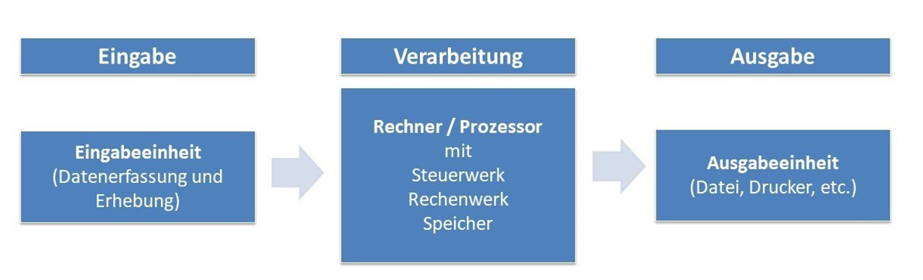
\includegraphics[width=\textwidth]{images/EVAPrinzip.png}
        \caption{EVA-Prinzip; Quelle [20]}
        \label{fig:eva}
    \end{figure}


Die Programmierung und Konfiguration der Siemens-SPS erfolgt über das \textbf{Totally Inte
grated Automation Portal} (TIA Portal), eine integrierte Entwicklungsumgebung, die
verschiedene Automatisierungskomponenten wie SPS, HMI und Antriebstechnik vereint.
Das TIA Portal unterstützt die Programmiersprachen gemäß \textbf{IEC 61131-3}, darunter
\textbf{Kontaktplan} (KOP), \textbf{Funktionsplan} (FUP), \textbf{Anweisungsliste} (AWL) und \textbf{Structured
Control Language} (SCL). Diese Vielfalt ermöglicht eine anwendungsorientierte und
normgerechte Entwicklung von Steuerungsprogrammen.[12]

    \begin{figure}[H]
        \centering
        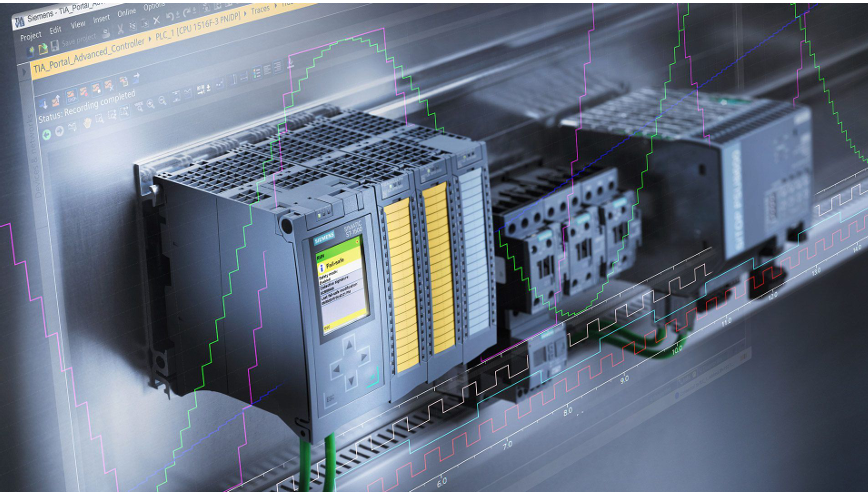
\includegraphics[width=\textwidth]{images/S7-1500.png}
        \caption{Beispiel S7-1500; Quelle [19]}
        \label{s7-1500}
    \end{figure}

Ein wesentliches Merkmal der \textbf{Siemens-SPS-Systeme} ist ihre Kompatibilität mit modernen Kommunikationsstandards wie \textbf{PROFINET} und \textbf{PROFIBUS}. Dadurch wird ei
ne nahtlose Integration in industrielle Netzwerke gewährleistet. Im Kontext von \textbf{Industrie 4.0} kommt den Siemens-SPS eine Schlüsselrolle zu, da sie die Grundlage
für intelligente, vernetzte und adaptive Produktionssysteme bilden. Die Fähigkeit zur
\textbf{Echtzeit-Datenerfassung und-verarbeitung} sowie zur Anbindung an Cloud- und
\textbf{IoT-Plattformen} macht sie zu einem integralen Bestandteil digitalisierter Fertigungspro
zesse.[22

\subsubsection{SPS-Programmierung}
In der Automatisierungstechnik werden speicherprogrammierbare Steuerungen (SPS)
zur Realisierung unterschiedlichster Abläufe eingesetzt. Um die gewünschten Funktio
nen zur Automatisierung von Prozessen umzusetzen, ist es erforderlich, diese Abläufe
in Form eines Programms in die Steuerung zu implementieren.
Ein SPS-Programm folgt dabei in der Regel einem klar strukturierten Aufbau [16]:

\begin{itemize}
    \item Definition der Ein-, Ausgangs- und Hilfsvariablen in einer Variablentabelle,
    
    \item Programmierung des Hauptprogramms mit den zugehörigen Unterprogrammen und Funktionsbausteinen,

    \item Kompilierung des Programms und Übertragung in die Steuerung.
\end{itemize}


    \begin{figure}[H]
        \centering
        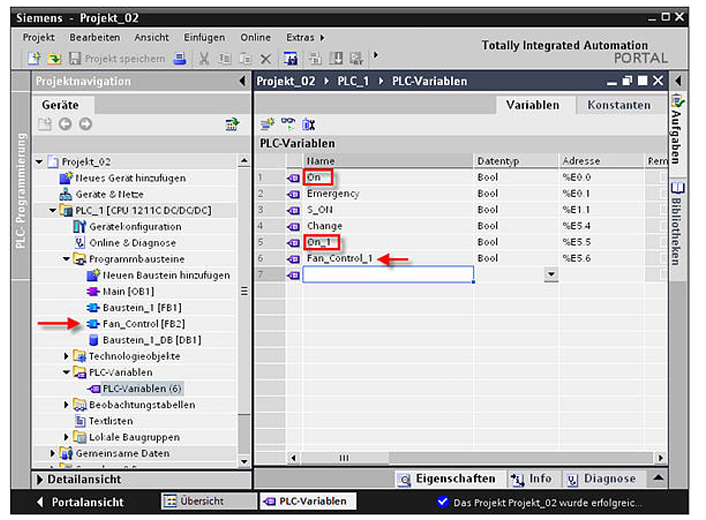
\includegraphics[width=\textwidth]{images/VariablentabelleTIA.png}
        \caption{Übersicht der Variablentabelle in TIA Portal [18]}
        \label{vartabtia}
    \end{figure}


Das Hauptprogramm besteht aus sogenannten \textbf{POUs} (Program Organization Units,
deutsch: Programmorganisationseinheiten). Diese werden in drei Arten unterteilt: \textbf{Pro
gramme}, \textbf{Funktionen} (FC) und \textbf{Funktionsbausteine} (FB). Die Realisierung dieser
POUs in Siemens TIA Portal wurde bereits im vorherigen Kapitel \ref{XXXXXXXXX} beschrieben.

Nachfolgend wird die Bedeutung und Funktion der einzelnen Organisationseinheiten
erläutert.


Das \textbf{Programm} dient der Realisierung komplexer Abläufe, beispielsweise von Schrittket
ten oder Hauptlogiken. Eine \textbf{Funktion} (FC) ist mit einer C-ähnlichen Funktion vergleich
bar. Sie verarbeitet eine oder mehrere Eingangsvariablen und gibt nach der Abarbeitung
ein Ergebnis zurück. Gemäß IEC 61131-3 können Funktionen jedoch nicht rekursiv
aufgerufen werden und besitzen kein eigenes Speicherverhalten, d.h. sie können kei
ne Werte dauerhaft speichern [16]. Ein einfaches Beispiel hierfür ist ein logisches
\textbf{UND-Gatter}.
Ein \textbf{Funktionsbaustein} (FB) hingegen besitzt ein internes Gedächtnis und kann Werte
über mehrere Zyklen hinweg speichern. Dadurch eignet er sich besonders für Zu
standsautomaten oder speichernde Operationen. Ein klassisches Beispiel hierfür ist ein
\textbf{RS-Flip-Flop}.


Für die Programmierung stehen verschiedene Sprachen nach IEC 61131-3 [1] zur
Verfügung:

\begin{itemize}
    \item \textbf{KOP} (Kontaktplan),
    \item \textbf{AWL} (Anweisungsliste),
    \item \textbf{FUP/FBS} (Funktionsplan / Funktionsbausteinsprache),
    \item \textbf{ST/SCL} (Structured Text / Structured Control Language)1
\end{itemize}


In modernen Industrieanlagen werden überwiegend FUP und ST eingesetzt. Diese
Programmiersprachen zeichnen sich durch eine gute Übersichtlichkeit und eine effizi
ente Fehleranalyse aus. Trotzdem bestehen zwischen beiden Varianten wesentliche
Unterschiede, die in Tabelle 2 dargestellt sind.


\begin{center}
    % Erzeugt eine normale Tabellenbeschriftung ohne \begin{table}

    \begin{tabular}{|p{6cm}|p{6cm}|}
        \hline
            \textbf{ST / SCL (Structured Text / Structured Control Language)}  & \textbf{FUP (Funktionsplan)}\\
            \hline
            Textbasierte Programmiersprache & Grafische Programmiersprache\\
            \hline
            Hochsprachenähnlich (z.B. C, Pascal) & Verwendung grafischer Symbole und logischer Verknüpfungen\\
            \hline
            Klare und kompakte Struktur & Gefahr der Unübersichtlichkeit bei komplexen Programmen\\
            \hline
            Besonders geeignet für mathematische und logische Operationen & Gut geeignet für einfache logische Abläufe\\
            \hline
    \end{tabular}

    \captionof{table}{Vergleich zwischen ST (Structured Text) und FUP (Funktionsplan) [17]}
    \label{tab:VergleichSclFup}
\end{center}


1 \textbf{SCL} ist die Siemens-spezifische Implementierung der nach IEC 61131-3 genormten Programmierspra
che Structured Text (ST) im TIA Portal [13].
\ref{XXX}



Wie aus der Tabelle hervorgeht, bietet die textbasierte Programmiersprache \textbf{ST} ins
besondere bei komplexen Strukturen und mathematischen Berechnungen erhebliche
Vorteile. \textbf{FUP} hingegen ist für Einsteiger leichter verständlich und eignet sich für über
schaubare Steuerungslogiken. Mit zunehmender Komplexität der Abläufe stößt FUP
jedoch schnell an seine Grenzen, da die grafische Darstellung umfangreicher Strukturen
unübersichtlich werden kann [17]. Um die genauen Unterschiede zu erläutern, sollen
zunächst grundlegende Elemente der einzelnen Sprachen eingeführt werden. Zunächst
erfolgt eine Beschreibung der wichtigsten Grundbausteine in FUP.


\textbf{Wichtige Grundfunktionen (UND, ODER, NICHT) in FUP}


\begin{figure}[htbp]
  \centering
  \begin{subfigure}[b]{0.31\textwidth}
    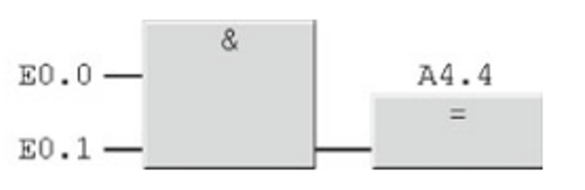
\includegraphics[width=\textwidth]{images/UndGatter.png}
    \caption{\textbf{UND-Gatter} [11]}
    \label{fig:undgatter}
  \end{subfigure}
  \hfill % Fügt flexiblen Abstand zwischen den Bildern ein
  \begin{subfigure}[b]{0.31\textwidth}
    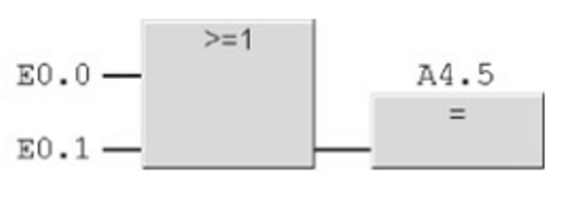
\includegraphics[width=\textwidth]{images/OderGatter.png}
    \caption{\textbf{ODER-Gatter} [11]}
    \label{fig:odergatter}
  \end{subfigure}
  \hfill
  \begin{subfigure}[b]{0.31\textwidth}
    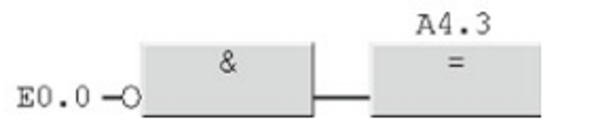
\includegraphics[width=\textwidth]{images/NotGatter.png}
    \caption{\textbf{NOT-Gatter} [11]}
    \label{fig:notgatter}
  \end{subfigure}
  
  \caption{Darstellung der logischen Grundfunktionen in FUP}
  \label{grundfufup}
\end{figure}


\textbf{Wichtige Funktionsbausteine in FUP}


\begin{figure}[htbp]
  \centering
  \begin{subfigure}[b]{0.49\textwidth}
    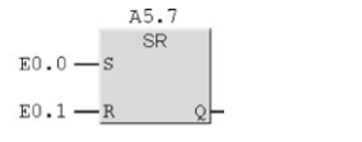
\includegraphics[width=\textwidth]{images/SRFlipFlop.png}
    \caption{\textbf{SR-FLIPFLOP} [11]}
    \label{fig:srflipflop}
  \end{subfigure}
  \hfill % Fügt flexiblen Abstand zwischen den Bildern ein
  \begin{subfigure}[b]{0.49\textwidth}
    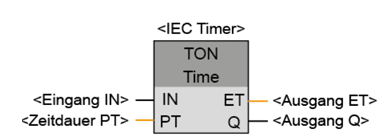
\includegraphics[width=\textwidth]{images/TON.png}
    \caption{\textbf{Einschaltverzögerung (TON)} [11]}
    \label{fig:ton}
  \end{subfigure}
  
  \caption{ Darstellung wichtiger Funktionsbausteine in FUP}
  \label{wichfunkbaust}
\end{figure}


In den obigen Abbildungen sind die wichtigsten Grundfunktionen und Funktionsbau
steine in \textbf{FUP} dargestellt. Mit diesen können diverse Abläufe realisiert werden, wie
beispielsweise einfache Förderbandsteuerungen. Komplexe, lange Abläufe sind jedoch
sehr aufwendig zu realisieren. Für eine SPS ist es daher gebräuchlich, hierfür auf
\textbf{ST/SCL} auszuweichen. In FUP können ebenfalls mathematische Operationen durch
geführt werden. Für Berechnungen existieren spezielle Bausteine. Allerdings ist es
schwierig, längere Rechenvorgänge übersichtlich darzustellen, da die Struktur schnell
unübersichtlich wird. Aus diesem Grund werden für sämtliche mathematische Opera
tionen häufig Berechnungen in \textbf{ST/SCL} durchgeführt. Beim vorliegenden Modell, dem
Hochregallager, wurde beispielsweise die Positionsermittlung der Lagerplätze für das
automatisierte Einlagern im vergangenen Studienprojekt in \textbf{SCL} realisiert.

\textbf{Grundlegende Anweisungen in SCL}


Im vorliegenden Projekt wird mit einer Siemens SPS gearbeitet. Somit ist SCL (Structu
red Control Language) der Standard im Bereich textbasierte Programmierung.
Hierbei gibt es einige konkrete Anweisungen, welche eine übersichtliche Programmie
rung gewährleisten.

Zu diesen zählen:

    \begin{itemize}
        \item \textbf{Zuweisungen:} Variable := Wert; Beispiel: Motor\_Start := TRUE;
        
        \item \textbf{Bedingte Anweisungen (IF-Strukturen):} IF Sensor = TRUE THEN Motor := TRUE; END\_IF;
        
        \item \textbf{Mehrzweigige Bedingungen (IF-ELSIF-ELSE):} IF Temp > 50 THEN Alarm := TRUE; ELSIF Temp > 30 THEN Warning := TRUE; ELSE Alarm := FALSE; END\_IF;
        
        \item \textbf{Schleifenstrukturen:} FOR i := 1 TO 5 DO Count := Count + 1; END\_FOR
        
        \item \textbf{Vergleiche und logische Operatoren:} AND, OR, NOT, >, <, =, >=, <=
        
    \end{itemize}

Diese Anweisungen ermöglichen selbst komplexe Programme zu realisieren. Es können
mathematische Berechnungen deutlich einfacher durchgeführt werden als beispielsweise in der Programmiersprache \textbf{FUP}.


\textbf{Vergleich SCL- FUP}


Die Programmiersprachen \textbf{FUP} und \textbf{SCL} werden beide für die Programmierung spei
cherprogrammierbarer Steuerungen verwendet.

Da \textbf{SCL} eine Siemens-eigene Sprache ist, konzentriert sich dieser Vergleich ausschließlich auf \textbf{STEP 7}.
Wie bereits erwähnt, ermöglicht \textbf{FUP} eine einfache blockbasierte Programmierung.
\textbf{FUP} eignet sich besonders für einfache Anwendungen, wie beispielsweise die Ansteue
rung von Drehstrommotoren. Auch für einfache Schrittketten ist \textbf{FUP} gut geeignet.
Mit zunehmender Programmkomplexität leidet jedoch die Übersichtlichkeit, was zu einer
erhöhten Fehleranfälligkeit führen kann.
Um diese Probleme zu vermeiden, wird in großen Produktionsanlagen mit komplexen Abläufen überwiegend textbasiert, also in \textbf{SCL}, programmiert. Die folgenden Darstellungen vergleichen beide Sprachen und verdeutlichen ihre Unterschiede. Dargestellt ist
eine einfache Förderbandsteuerung in \textbf{FUP} und \textbf{SCL} im TIA Portal.



\begin{figure}[htbp]
  \centering
  \begin{subfigure}[b]{0.49\textwidth}
    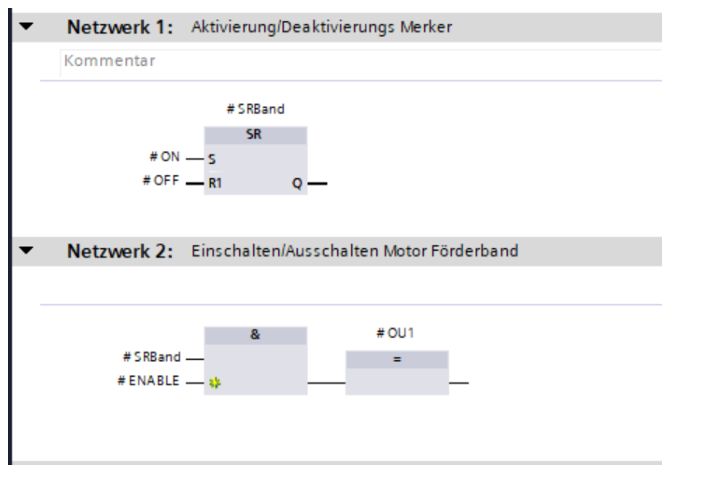
\includegraphics[width=\textwidth]{images/FBSteuerungFoerderband.png}
    \caption{Funktionsbaustein zur Steuerung des Förderbands}
    \label{fig:fbsteuerungfoeba}
  \end{subfigure}
  \hfill % Fügt flexiblen Abstand zwischen den Bildern ein
  \begin{subfigure}[b]{0.49\textwidth}
    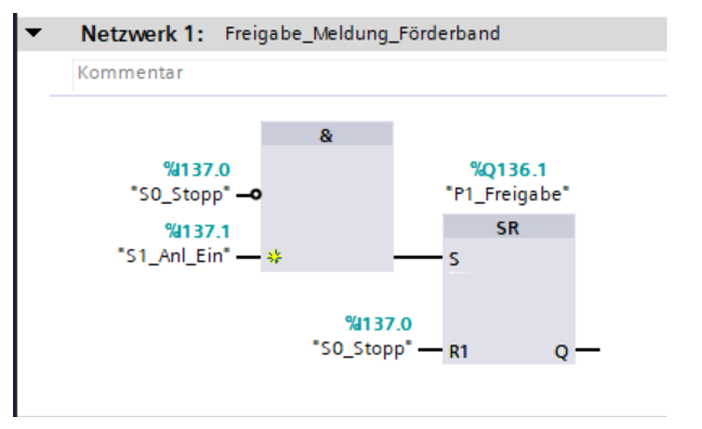
\includegraphics[width=\textwidth]{images/FreigabeImOB.png}
    \caption{Freigabe im Haupt-OB}
    \label{fig:freigahauptob}
  \end{subfigure}
  
  \caption{Realisierung der Förderbandsteuerung in FUP}
  \label{foebafup}
\end{figure}


\begin{figure}[htbp]
  \centering
  
  % Linker Codeblock (a)
  \begin{subfigure}[t]{0.45\textwidth}
\begin{lstlisting}
IF #OFF THEN
    #SR_Band := FALSE;
ELSIF #ON THEN
    #SR_Band := TRUE;
END_IF;

#OU1 := #SR_Band AND #ENABLE;

\end{lstlisting}
    \caption{SCL-Code des Förderband-Bausteins}
    \label{fig:scl_baustein}
  \end{subfigure}
  \hfill
  % Rechter Codeblock (b)
  \begin{subfigure}[t]{0.50\textwidth}
\begin{lstlisting}
IF NOT "S0_Stop" AND "S1_Anl_Ein" THEN
    "P1_Freigabe" := TRUE;
ELSIF "S0_Stop" THEN
    "P1_Freigabe" := FALSE;
END_IF;

"Foerderband"(
  OFF    := "B2_vorne",
  ON     := "B1_hinten",
  ENABLE := "P1_Freigabe",
  OU1    => "Q1_Band");

\end{lstlisting}
    \caption{Aufruf des Förderband-Bausteins im Hauptprogramm}
    \label{fig:scl_aufruf}
  \end{subfigure}

  \caption{Realisierung des Förderbandprogramms in \textbf{SCL}}
  \label{foerderband_scl}
\end{figure}

\clearpage

Anhand des Beispiels mit den Abbildungen \ref{foebafup} und \ref{foerderband_scl} wird deutlich, dass \textbf{FUP} auf den ersten Blick leichter
verständlich wirkt, da es sich um die grafische Verschaltung logischer Funktionen
handelt.
Auf den zweiten Blick zeigt sich jedoch, dass der Programmieraufwand deutlich höher
ist als in \textbf{SCL}. In \textbf{SCL} kann dieselbe Funktionalität mit wenigen, klar strukturierten
Codezeilen realisiert werden, ohne das Programm mit zusätzlichen Netzwerken zu
überladen.
Zusammenfassend lässt sich festhalten, dass sowohl \textbf{FUP} als auch \textbf{SCL} ihre jeweiligen
Vor- und Nachteile besitzen. Je nach Anwendung und Komplexität des Prozesses fällt
die Entscheidung für die eine oder die andere Programmiersprache

\subsubsection{Industrielle Bussysteme}
In der Automatisierung sind Kommunikationsprotokolle entscheidend für die Vernetzung
einzelner Systeme. Die Funktionalität einer automatisierten Anlage basiert auf der
erfolgreichen Kommunikation der einzelnen Komponenten.
Bussysteme in der Automatisierungstechnik
Ein großer Bestandteil im Bereich der Kommunikation zwischen verschiedenen Teilneh
mern bilden sogenannte Bussysteme.
Sie kommen zum Einsatz, wenn eine Steuerung mit den Sensoren bzw. Aktoren eines
Systems effizient kommunizieren soll. Die Steuerung kann z.B. eine \textbf{SPS} oder ein
\textbf{Mikrocontroller} sein.
Früher wurden Signale hauptsächlich über Hartverdrahtung übertragen. Diese Methode
war zwar zuverlässig, jedoch sehr aufwändig zu implementieren und mit hohem Material
und Zeitaufwand verbunden.
Deshalb wurden die bereits erwähnten Bussysteme eingeführt. Mit deren Hilfe ist es
möglich, mit geringem Verdrahtungsaufwand mit mehreren Teilnehmern innerhalb eines
Systems zu kommunizieren.
Ein Bussystem besteht grundsätzlich aus einer Leitung, über die mehrere Teilnehmer
angesprochen werden können. Die Topologie ist hierbei vielfältig. Es gibt sogenannte
\textbf{Stern-}, \textbf{Linien-} oder auch \textbf{Ring-Topologien}.


    \begin{figure}[H]
        \centering
        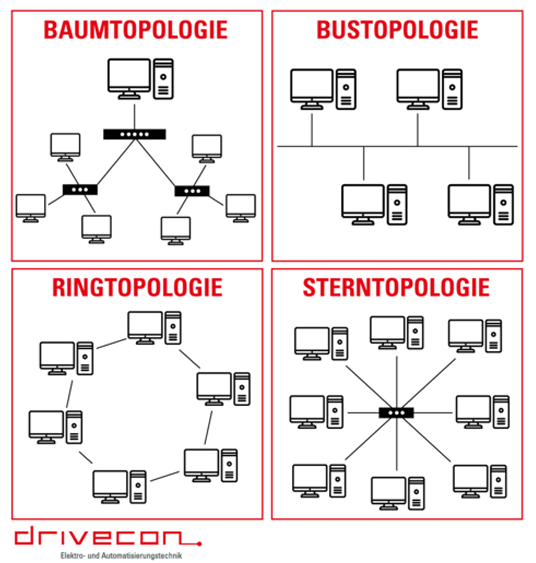
\includegraphics[width=\textwidth/2]{images/BusTopologien.png}
        \caption{Gängige Bus- Topologien; Quelle [6]}
        \label{bustopologien}
    \end{figure}


Die am häufigsten angewandte Methode ist die Kommunikation über eine \textbf{Linientopologie}.
Hierbei werden mehrere Teilnehmer über einzelne Abzweige nacheinander angesteuert.
Bussysteme können auf den verschiedensten Ebenen der Automatisierungspyramide[5]
zum Einsatz kommen. Der Haupteinsatz erfolgt jedoch auf der Feld- und Steuerungs
ebene.
Weiterhin gibt es verschiedene Arten von Bussystemen, die sich in ihrer Struktur, Ge
schwindigkeit und Übertragungsart unterscheiden. Die am häufigsten verwendeten sind
im Folgenden aufgelistet:

\begin{itemize}
    \item Feldbus-basierte Kommunikationssysteme (z.B. \textbf{Profibus})
    
    \item Ethernet-basierte Kommunikationssysteme (z.B. \textbf{PROFINET})
    
    \item Punkt-zu-Punkt-Systeme (z.B. \textbf{IO-Link})
\end{itemize}


Im Folgenden eine kurze Gegenüberstellung der einzelnen Protokolle:


\begin{center}
    % Erzeugt eine normale Tabellenbeschriftung ohne \begin{table}

    \begin{tabular}{|p{4cm}|p{3.5cm}|p{3.5cm}|p{3.5cm}|}
        \hline
            \textbf{Kriterium} & \textbf{IO-Link} &\textbf{PROFINET} &\textbf{PROFIBUS}\\
            \hline
            \textbf{Kommunikations- prinzip} & Punkt-zu-Punkt (PTP) & Ethernet-basiert& Feldbus-basiert \\
            \hline
            \textbf{Topologie}& Baum & Linie, Stern, Ring & Linie, Baum\\
            \hline
            \textbf{Kommunikations- rate} &4,8/ 38,4/ 230,4k Baud & bis 100Mbit/s & bis 12Mbit/s\\
            \hline
            \textbf{Typische Anwendung} & Sensorik, Aktorik, Handhabungstechnik & Steuerung, Kommunikation, Anlagenvernetzung& Maschinensteuer., Antriebsregelung\\
            \hline
    \end{tabular}

    \captionof{table}{Vergleich der Kommunikationssysteme IO-Link, PROFINET und PROFIBUS; Quellen: [5][15][14]}
    \label{tab:vergleichIOlinkprofinetprofibus}
\end{center}

\subsubsection{IO-Link}
IO-Link ist ein Kommunikationssystem, welches der Anbindung intelligenter Sensoren
und Aktoren dient.
Es wurde entwickelt, um die Lücke zwischen Feldbussen und Industrial-Ethernet
Systemen zu schließen. Der Standard ist in der Norm IEC 61131-9 definiert. IO-Link
wird häufig in Fabrikautomatisierungsanlagen eingesetzt.

\textbf{Aufbau und Funktionsweise von IO-Link}
IO-Link ist ein Kommunikationssystem, das nach dem \textbf{Point-to-Point} (PTP)-Prinzip
arbeitet. Das bedeutet, es werden mehrere Teilnehmer Punkt zu Punkt angesteuert.

Der \textbf{IO-Link-Master} ist hierbei mit den \textbf{IO-Link-Devices} PTP-verbunden. Dieser stellt
die Schnittstelle zwischen der Steuerung (\textbf{SPS}) und der Sensor-/Aktor-Ebene dar.


    \begin{figure}[H]
        \centering
        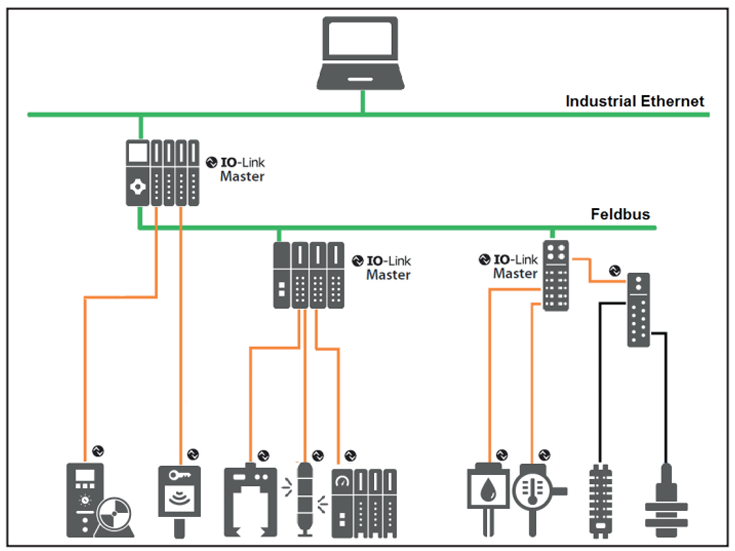
\includegraphics[width=350px]{images/IOLinkArchitektur.png}
        \caption{Architektur IO-Link; Quelle [5]}
        \label{}
    \end{figure}



Das System arbeitet \textbf{bidirektional}[5]. 
Das bedeutet, der IO-Link-Master kann sowohl
Prozessdaten empfangen als auch neue Parameter an die Devices senden (z.B. \textbf{RFID}).
Die Verbindung erfolgt über dreipolige Standardleitungen2.10. Dadurch lässt sich IO
Link problemlos in das Gesamtsystem integrieren. Eine separate Busverkabelung ist
nicht notwendig[2].


    \begin{figure}[H]
        \centering
        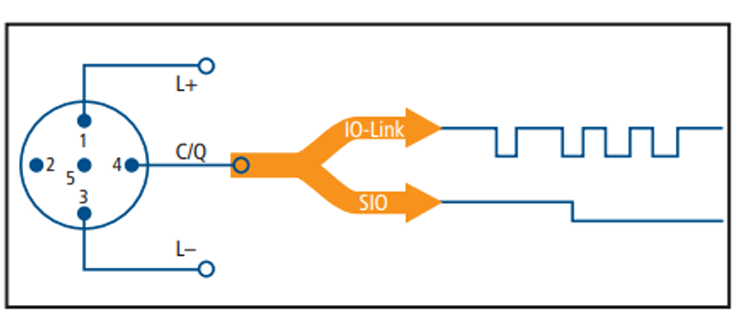
\includegraphics[width=500px]{images/IOLinkAnschluss.png}
        \caption{Anschlussbelegung IO-Link; Quelle [5]}
        \label{iolinkanschluss}
    \end{figure}

Der IO-Link-Master2.11 kann über ein übergeordnetes Bussystem (z.B. \textbf{Profibus},
\textbf{PROFINET}) mit der SPS kommunizieren[14].


    \begin{figure}[H]
        \centering
        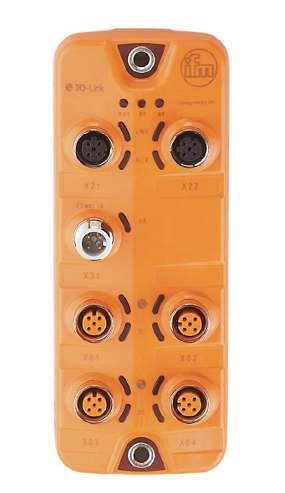
\includegraphics[width=\textwidth/3]{images/IOLinkMaster.png}
        \caption{Master IO-Link; Quelle [9]}
        \label{iolinkmaster}
    \end{figure}

\textbf{Kommunikation und Datenaustausch} Die Kommunikation über IO-Link erfolgt seriell. Hierbei wird mit festen Baudraten von 4,8kBaud, 38,4kBaud oder 230,4kBaud übertragen.
Die Datenkommunikation gliedert sich in drei Hauptarten[5]:

\begin{itemize}
    \item \textbf{Prozessdaten}:
    Diese werden zyklisch zwischen Master und Device ausgetauscht. Sie enthalten
    z. B. Messwerte von Sensoren oder Schaltzustände von Aktoren.
    \item \textbf{Servicedaten (Parameterdaten)}:
    Sie werden azyklisch übertragen und dienen zur Parametrierung oder Konfigu
    ration der Geräte. So können beispielsweise Schaltpunkte, Messbereiche oder
    Filterzeiten direkt über die Steuerung angepasst werden.
    \item \textbf{Ereignisdaten}:
    Hierbei handelt es sich um Status- oder Fehlermeldungen, die das Device bei
    bestimmten Zuständen (z. B. Übertemperatur, Kabelbruch oder Spannungsfehler)
    an den Master sendet.
\end{itemize}

Durch diese Aufteilung ist eine gezielte Überwachung, Diagnose bei Fehlern und
Konfiguration der einzelnen Module möglich. Eine Prozessunterbrechung ist hierfür
nicht notwendig.

Auf Protokollebene wird zwischen drei Schichten unterschieden[5]:


\begin{itemize}
    \item \textbf{Physikalische Schicht}: Definiert die elektrische Verbindung über die dreipolige Leitung.

    \item \textbf{Datenverbindungsschicht}: Regelt das Telegrammformat und die Fehlererkennung.

    \item \textbf{Applikationsschicht}: Beschreibt den Austausch von Prozess-, Service- und Ereignisdaten.
\end{itemize}


\textbf{Komponenten eines IO-Link-Systems}


Ein vollständiges IO-Link-System besteht in der Regel aus folgenden Komponenten[5]:

\begin{itemize}
    \item \textbf{IO-Link-Master}: Er verwaltet die Kommunikation zu den einzelnen IO-Link-Devices und bildet die Schnittstelle zur übergeordneten Steuerung. Je nach Ausführung kann der Master als Schaltschrankmodul oder als Feldmodul ausgeführt sein. Letzteres wird direkt in der Anlage montiert, wodurch sich Installationsaufwand und Verkabelungslänge reduzieren.
    
    \item \textbf{IO-Link-Devices}: Hierbei handelt es sich um Sensoren, Aktoren oder andere Feldgeräte, die über IO-Link kommunizieren. Typische Beispiele sind Drucksensoren, Wegmesssysteme, Ventilinseln, RFID-Leseeinheiten oder Smart Lights. Jedes Device verfügt über eine IODD-Datei (IO Device Description), in der alle Geräteparameter, Kom
    munikationsdaten und Diagnosemöglichkeiten beschrieben sind. Diese Datei wird
    im Engineering-Tool der Steuerung verwendet, um das Gerät automatisch zu
    erkennen und korrekt zu parametrieren.

    \item \textbf{Verkabelung}:
    IO-Link nutzt standardisierte, ungeschirmte Leitungen mit M12- oder M8-Steckverbindern.
    Die Kabellängen betragen typischerweise bis zu 20m zwischen Master und Device.
    Da das Signal digital übertragen wird, ist die Verbindung unempfindlich gegenüber
    elektromagnetischen Störungen und Spannungsabfällen.
\end{itemize}

\textbf{Zusammenfassung}

Über IO-Link ist eine Kommunikation bis in die unterste Feldebene möglich. Analoge
Signale sind hierbei überflüssig, da die Schnittstelle standardisiert ist. Weiterhin lassen
sich Geräte identifizieren und parametrieren. Außerdem stehen umfassende Diagno
semöglichkeiten zur Verfügung.
Damit trägt IO-Link wesentlich zur Transparenz, Flexibilität und Wartungsfreundlich
keit moderner Automatisierungssysteme bei und bildet eine wichtige Grundlage für
Konzepte wie \textbf{Industrie 4.0}[5].


\subsubsection{Vorteile und Nutzen in der Praxis}
Der Einsatz von IO-Link in der Industrie bringt zahlreiche Vorteile mit sich. Es werden
technische Defizite von klassischen Bus- und Anschlusssystemen eliminiert. Neben der
Vereinfachung der Verdrahtung bietet das System eine hohe Flexibilität, verbesserte
Diagnosefähigkeiten sowie eine sehr gute digitale Kommunikation bis in die Feldebene
hinein.

Durch die genannten Punkte wird nicht nur die Leistungsfähigkeit der Anlage gesteigert,
sondern auch die Wirtschaftlichkeit und Nachhaltigkeit in einer Produktion verbessert.


\textbf{Technische Vorteile}
Ein zentraler technischer Vorteil von IO-Link besteht in der vollständig digitalen Signal
übertragung zwischen dem IO-Link-Master und den angeschlossenen Devices. Dadurch
entfallen typische Nachteile analoger Schnittstellen wie Messfehler durch Spannungsab
fall, Rauschen oder Kalibrierungsabweichungen. Jeder über IO-Link verbundene Sensor
oder Aktor überträgt exakte Prozessdaten in digitaler Form, wodurch die Messqualität
und Zuverlässigkeit deutlich erhöht werden.
Ein weiterer Vorteil ist die sogenannte bidirektionale Kommunikation. Hierbei ist es
möglich, dass der IO-Link-Master Daten empfangen kann, sowie in der Lage ist, die
Parameter der Sensoren oder Aktoren zu beschreiben.
Darüber hinaus bietet IO-Link standardisierte Schnittstellen und Datenstrukturen, die
herstellerübergreifend kompatibel sind. Jedes Gerät wird anhand seiner IODD-Datei (IO
Device Description) automatisch erkannt, was die Integration in bestehende Systeme
erheblich vereinfacht[5]. Diese Einheitlichkeit führt zu einer hohen Austauschbarkeit der
Komponenten, ohne dass Änderungen in der SPS-Software oder in der Verdrahtung
notwendig sind.


\textbf{Weitere Vorteile}



Durch den verringerten Verdrahtungsaufwand können erhebliche Kosten eingespart
werden. Diese können an anderer Stelle effizienter eingesetzt werden.
Da ein IO-Link-Master in der Lage ist, sowohl klassische als auch digitale Signale zu
verarbeiten, entfallen zusätzliche Baugruppen zur Verarbeitung bestimmter Signalarten.
Diese Punkte führen zu einer Erhöhung bzw. Verbesserung der Wirtschaftlichkeit.
Dadurch kann nachhaltiger und effektiver gearbeitet werden.


\textbf{Erweiterte Diagnosemöglichkeiten}


Eine besondere Eigenschaft von IO-Link liegt in den umfassenden Diagnosemöglichkeiten, die dem Anwender zur Verfügung stehen. Jedes Device ist in der Lage, sich selbst
zu diagnostizieren und die entsprechenden Informationen an den \textbf{IO-Link-Master} zu
übermitteln.
Somit werden Fehler wie Kabelbruch, Kurzschluss oder Unterspannung sofort an die
Steuerung gemeldet. Dadurch ist ein schnelles und effektives Trouble Monitoring ge
geben. Dies führt dazu, dass langfristig Fehlerquellen und Anfälligkeiten in Systemen
erkannt und gezielt beseitigt werden können.


\textbf{Praxisbeispiel}


In der industriellen Praxis findet IO-Link zunehmend Anwendung bei intelligenten Sen
soren und Aktoren, etwa in Montage- und Prüfprozessen oder bei der Handhabungs
technik.
Ein typisches Beispiel ist die Integration eines IO-Link-Füllstandssensors oder Druck
sensors in ein SPS-System. Die Messwerte werden dabei digital und störungsfrei
übertragen, während gleichzeitig Geräteparameter über die Steuerung angepasst wer
den können, etwa der Schaltpunkt oder der Messbereich[5].



\textbf{Zusammenfassung}


IO-Link vereint einfache Installation mit intelligenter Kommunikation. Die Technologie
schafft eine durchgängige Datenbasis von der Feldebene bis zur Steuerung und ermög
licht so eine effiziente, flexible und zukunftssichere Automatisierung.
Durch die Kombination aus digitaler Signalübertragung, erweiterter Diagnose und au
tomatischer Parametrierung wird IO-Link zu einem zentralen Bestandteil moderner
Industrie-4.0-Architekturen.


\subsubsection{Sicherheit in der Automatisierung}
m Kontext der Automatisierung von technischen Anlagen ist die Sicherheit der größte
und wichtigste Aspekt [4].
Beim Betreiben eines Systems muss vollständig ausgeschlossen sein, dass keine
Gefahr für Menschen, von der Anlage, ausgeht. Das bedeutet, bei Planung der Anlage,
steht die Sicherheit im Fokus.
Speziell in der Produktion bzw. in der Logistik sind sicherheitstechnische Aspekte enorm
wichtig.
Bei automatisierten Prozessen wie z.B. das Verfahren eines Hochregallagers, können
Gefahren durch Implementierung von Sicherheitslogiken ausgeschlossen werden.
Das Ziel ist immer Gefährdungen bzw. Verletzungen von Menschen zu verhindern.


\textbf{Einordnung in den Kontext der funktionalen Sicherheit}

Um die Sicherheitsprinzipien besser zu verstehen, ist es wichtig, die einzelnen Aspekte
der Sicherheitsthematik im Gesamtkontext einzuordnen.
In diesem Zusammenhang spielt der Bereich der funktionalen Sicherheit eine entschei
dende Rolle.
Hierunter versteht man den Teil einer Maschine, der von den korrekt funktionierenden
Steuerungs- und Sicherheitskomponenten abhängt. Sie sorgt dafür, dass bei kritischen
Situationen ein sicherer Zustand der Anlage erreicht wird. Ein Beispiel hierfür wäre das
direkte Abschalten eines Motors[10].
Damit sicherheitsbezogene Steuerungssysteme zuverlässig arbeiten, müssen sie be
stimmte Anforderungen erfüllen, die in internationalen Normen festgelegt sind.


Einige dieser Vorschriften sind im Folgenden aufgelistet[10]:

\begin{itemize}
    \item \textbf{ENISO13849-1}: Beschreibt die sicherheitsrelevanten Teile einer Anlage, unter anderem den \textbf{PL} (Performance Level).
    \item \textbf{IEC 61508}: Behandelt die funktionale Sicherheit elektrischer, elektronischer und programmierbarer Steuerungssysteme. Basiert auf dem \textbf{SIL} (Safety Integrity Level).
    \item \textbf{EN61496}: Sicherheit von Maschinen– Berührungslos wirkende Schutzeinrichtungen (BWS), beispielsweise Lichtschranken oder Lichtvorhänge.
\end{itemize}

Die genannten Normen zeigen ebenfalls die Bedeutung der Sicherheit im Anlagenbau
für den Gesetzgeber. Falls es zu Verstößen kommen sollte, führt dies zu Konsequenzen
für den Arbeitgeber.
Das ist der Grund dafür, dass Unternehmen sehr genau auf die Einhaltung dieser
Vorschriften achten.
Für die genannten Normen gibt es dementsprechende Geräte, welche beispielsweise
im Fehlerfall (Fehlerstrom) abschalten sollen (FI-Schutzschalter).
Die Auswahl der Sicherheitskomponenten erfolgt auf Basis einer sogenannten \textbf{Risiko
beurteilung}. Diese ermittelt die potenziellen Gefahren und legt das \textbf{Performance Level}
bzw. den \textbf{SIL} fest. In der Praxis werden Sicherheitsfunktionen häufig mit einem \textbf{PL d}
oder \textbf{SIL 2} realisiert, da diese ein gutes Verhältnis zwischen Aufwand und Sicherheit
bieten.


Eine zentrale Rolle innerhalb dieser sicherheitsrelevanten Systeme spielt die \textbf{Sensorik}.
Sie dient als Grundlage zur Erfassung von Zuständen und Bewegungen innerhalb einer
Anlage und bildet somit die Basis für jede Sicherheitsfunktion.
Besonders in automatisierten Prozessen ist es wichtig, dass Gefahrenzonen zuverlässig
überwacht werden, ohne den Produktionsablauf zu beeinträchtigen.


Hier kommen berührungslos wirkende Schutzeinrichtungen zum Einsatz, wie beispiels
weise \textbf{Lichtschranken} oder \textbf{Lichtvorhänge}. Diese ermöglichen eine sichere und
zugleich flexible Absicherung von Arbeitsbereichen, an denen Mensch und Maschine
aufeinandertreffen.
Lichtschranken zählen zu den am weitesten verbreiteten Sicherheitseinrichtungen in
der Industrie und werden unter anderem bei Robotersystemen, Förderanlagen oder
automatisierten Handhabungsstationen verwendet.
Im folgenden Abschnitt wird die Funktionsweise, der Aufbau sowie der Einsatz von
Lichtschranken in sicherheitsrelevanten Anwendungen näher erläutert.

\subsubsection{Lichtschranken in sicherheitsrelevanten Anlagen}
Die Lichtschranke ist eine der wichtigsten Sicherheitseinrichtungen in der Fertigung und
Logistik.
Sie verhindert das unbefugte Eingreifen in laufende Prozesse, sodass mögliche Gefah
ren für Personen zuverlässig ausgeschlossen werden können.
Viele Hersteller bieten ihre Bauteile frei konfigurierbar an. Dadurch ist es möglich,
die Betriebsmodi und Parameter individuell an die jeweilige Anwendung anzupassen,
beispielsweise bei der Absicherung von Hochregallagern oder automatisierten Förder
anlagen.
Lichtschranken kommen in sicherheitsrelevanten Anlagen überall dort zum Einsatz, wo
Gefahrenbereiche zuverlässig überwacht werden müssen, ohne dass mechanische
Barrieren den Prozessfluss behindern.


\textbf{Funktionalität einer Lichtschranke}


Bei einer Lichtschranke handelt es sich um eine berührungslos wirkende Schutzeinrichtung, die mit einem oder mehreren Lichtstrahlen arbeitet. Diese Lichtstrahlen bilden
eine optische Barriere, die bei Unterbrechung ein Signal auslöst.
Eine Lichtschranke besteht grundsätzlich aus zwei Modulen: einem \textbf{Sender} und einem
\textbf{Empfänger}. Der Sender erzeugt ein Lichtsignal, das vom Empfänger erfasst wird. 

Wird
der Lichtstrahl unterbrochen, erkennt die Auswerteelektronik diesen Zustand und leitet
eine vordefinierte Sicherheitsreaktion ein, beispielsweise das Abschalten eines Antriebs oder das Anhalten eines Roboters.
Die am häufigsten verwendeten Lichtschrankentypen sind die \textbf{Reflexionslichtschranke}
und die \textbf{Infrarotlichtschranke}[3].
Bei einer \textbf{Reflexionslichtschranke} befinden sich Sender und Empfänger im selben
Gehäuse. Das ausgesendete Lichtsignal wird über einen Reflektor zurückgeworfen und
von der Empfangseinheit detektiert. Wird der Lichtstrahl durch ein Objekt unterbrochen,
bleibt das Signal aus und die Sicherheitsfunktion wird aktiviert.

Die im Projekt verwendete Variante ist eine \textbf{Infrarotlichtschranke}. Diese arbeitet mit
unsichtbarem Infrarotlicht, das unempfindlich gegenüber Umgebungslicht und Staub ist.

    \begin{figure}[H]
        \centering
        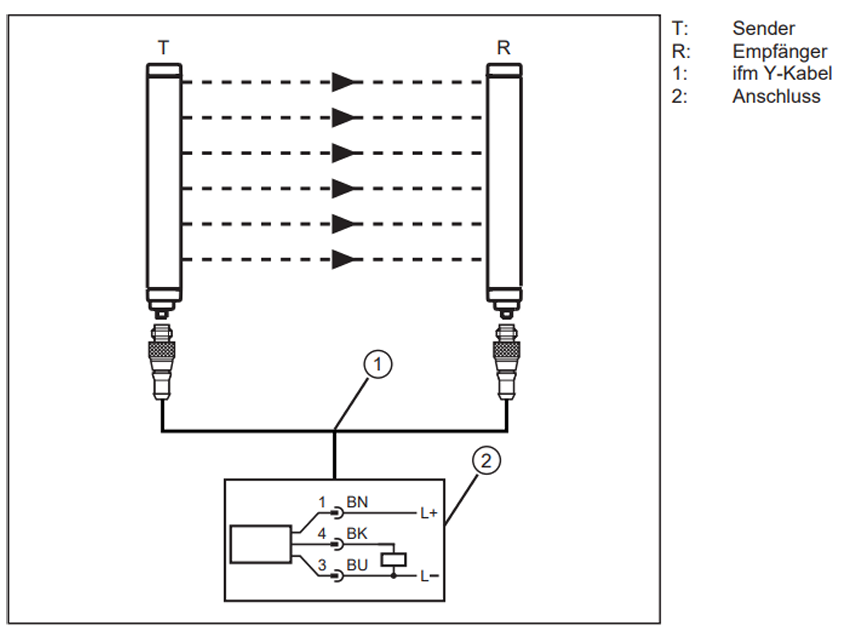
\includegraphics[width=350px]{images/SchematischeDarstellungIFMLichtgatter.png}
        \caption{Schematische Darstellung des IFM Lichtgatters[7]}
        \label{ifmlichtgatter}
    \end{figure}

Hierbei wird ein kontinuierlicher Infrarotstrahl vom Sender ausgesendet, der vom Empfänger registriert wird. Wird der Strahl unterbrochen, erkennt die Steuerung dies sofort
als Störung oder Eingriff und löst eine Sicherheitsreaktion aus 2.12.
Durch die hohe Reichweite und Störsicherheit eignet sich die Infrarotlichtschranke
besonders für industrielle Umgebungen, in denen eine präzise und zuverlässige Objek
terkennung gefordert ist.
Häufig variiert die Bezeichnung solcher Systeme. Viele Hersteller verwenden dafür auch
den Begriff \textbf{Lichtgitter} oder \textbf{Lichtvorhang}.
So auch der Hersteller \textbf{ifm}, der das im Projekt verwendete Produkt bereitstellt [8]. 

Diese
Systeme sind modular aufgebaut und lassen sich über verschiedene Schnittstellen
beispielsweise IO-Link direkt in eine Steuerung integrieren

